\documentclass[9pt]{beamer}
%\usetheme{CambridgeUS}
\usetheme{Antibes}
\usecolortheme[RGB={120,130,235}]{structure}

\usepackage{graphics}
\usepackage{marvosym}
\usepackage{graphicx}
\usepackage{latexsym}
\usepackage{amsmath}
\usepackage{amsfonts,amssymb}
\usepackage{ mathrsfs }
\usepackage{amsthm}
\usepackage{multimedia}
\usepackage{subcaption}
\usepackage{hyperref}
\usepackage{breqn}
\usepackage{wasysym}
\usepackage{xcolor}
\usepackage{ stmaryrd }
\usepackage{soul}
\newtheorem{prop}{Proposition}

%Define New Macros
%\input macros
\renewcommand\o{\omega}
\newcommand{\deriv}{\mbox{d}}
\newcommand{\Real}{\mathbb R}
\newcommand{\T}{\mathbb T}
\newcommand{\norm}[1]{\|#1\|}
\newcommand{\abs}[1]{\left\vert#1\right\vert}
\newcommand{\set}[1]{\left\{#1\right\}}
\newcommand{\subheading}[1]{\noindent \textbf{#1}}
\newcommand{\grad}{\nabla}
\newcommand{\diverg}{\textup{div} }
\newcommand{\jump}[1]{[#1]}
\newcommand{\limit}[2]{\lim_{#1 \rightarrow #2}}
\newcommand{\mollify}[1]{ \mathcal{J}_\epsilon #1 }
\newcommand{\conv}[2]{#1 \ast #2}
\newcommand{\D}{D}
\newcommand{\K}{\mathcal{K}}
\newcommand{\ineqtext}[1]{ ^{\text{\tiny #1}}}
\newcommand{\wknorm}[2]{\norm{#1}_{L^{#2,\infty}}}
%\newcommand{\wknorm}[2]{\abs{#1}_{L_w^{#2}}}
\newcommand{\wkspace}[1]{L^{#1,\infty}}
%\newcommand{\wkspace}[1]{L_w^{#1}}
\newcommand{\F}{\mathcal{F}}
\newcommand{\G}{\mathcal{G}}
\newcommand{\eps}{\epsilon}
\newcommand{\lap}{\Delta}

%Nancy's macros
\newcommand{\reg}[1]{#1^\epsilon}
\newcommand{\Lpr}[1]{L^{#1}(\mathbb{R}^n)}
\newcommand{\Lp}[1]{L^{#1}(\Omega)}
\newcommand{\intreal}{\int_{\mathbb{R}^2}\hspace{-8pt}}
\newcommand{\energy}{\mathcal{F}}
\newcommand{\modenergy}{\mathcal{E}_H}
\newcommand{\kernel}{\mathcal{K}}
\newcommand{\into}{\int_{D}}
\newcommand{\intot}{\int_{D_T}}
\newcommand{\ball}{B_n}
\newcommand{\balltime}{B_n\times [0,T]}

\newcommand{\brak}[1]{\langle #1 \rangle} 
\usepackage{url}
\makeatletter
\g@addto@macro{\UrlBreaks}{\UrlOrds}
\makeatother
\newcommand*{\vpointer}{\vcenter{\hbox{\scalebox{2}{\Huge\pointer}}}}


\DeclareMathOperator{\R}{\mathbb{R}}

\title[Final Presentation]{Scientific Computation of Two--Phase Ferrofluid Flows} 
\author[Final Presentation]{Gareth Johnson \\[.3cm] Faculty Adviser: Prof. Ricardo Nochetto } 
\institute[] 
{
	University of Maryland\\ 
	AMSC 664: Advanced Scientific Computing II\\ 
	Supported by Johns Hopkins University Applied Physics Lab
}
\date[May 2019]{May 15, 2019}


\begin{document}
\begin{frame}
	\titlepage
\end{frame}

\section{Introduction}
\begin{frame}{What is a Ferrofluid?}
	\centering
	\href{https://youtu.be/wHZDgSFzQ_s?t=12}{Awesome video of ferrofluids.}
\end{frame}

\begin{frame}{What is a Ferrofluid? (Backup)}
	\begin{minipage}{.6\paperwidth}
		A ferrofluid is a colloid of nanoscale ferromagnetic particles suspended in a carrier fluid such as oil, water, or an organic solvent.
	\end{minipage}%
	\begin{minipage}{.3\paperwidth}
		\centering
		\flushbottom
		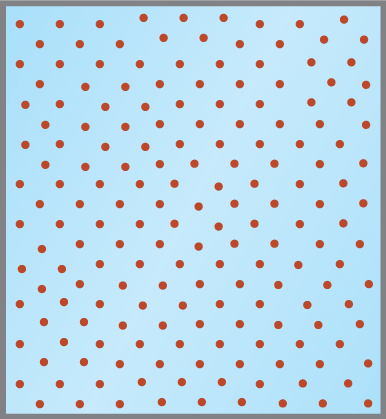
\includegraphics[scale=.5]{Colloid.jpg}
	\end{minipage}%
	\vspace{.3in}\\
	Ferrofluids become magnetized when under the effect of a magnetic field.
	\begin{minipage}{.4\paperwidth}
		\centering
		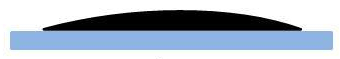
\includegraphics[scale=.3]{FerroStill.jpg}
	\end{minipage}%
	\begin{minipage}{.1\paperwidth}
		$\vpointer$
	\end{minipage}%
	\begin{minipage}{.3\paperwidth}
		\centering
		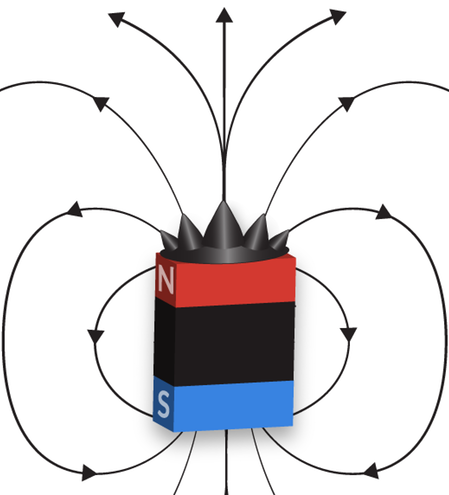
\includegraphics[scale=.18]{FerroExplain.png}
	\end{minipage}
\end{frame}

\begin{frame}{Applications}
	\begin{itemize}
		\item Initially created to pump rocket fuel once a spacecraft entered a weightless environment.
		\begin{minipage}{.5\paperwidth}
			\item Commercial applications:
			\begin{itemize}
				\item Vibration damping
				\item Sensors
				\item Acoustics
			\end{itemize}
			\item Recent research areas:
			\begin{itemize}
				\item Magnetic drug targeting
				\item Adaptive deformable mirrors
			\end{itemize}
		\end{minipage}%
		\begin{minipage}{.3\paperwidth}
			\begin{figure}[!b]
				\centering
				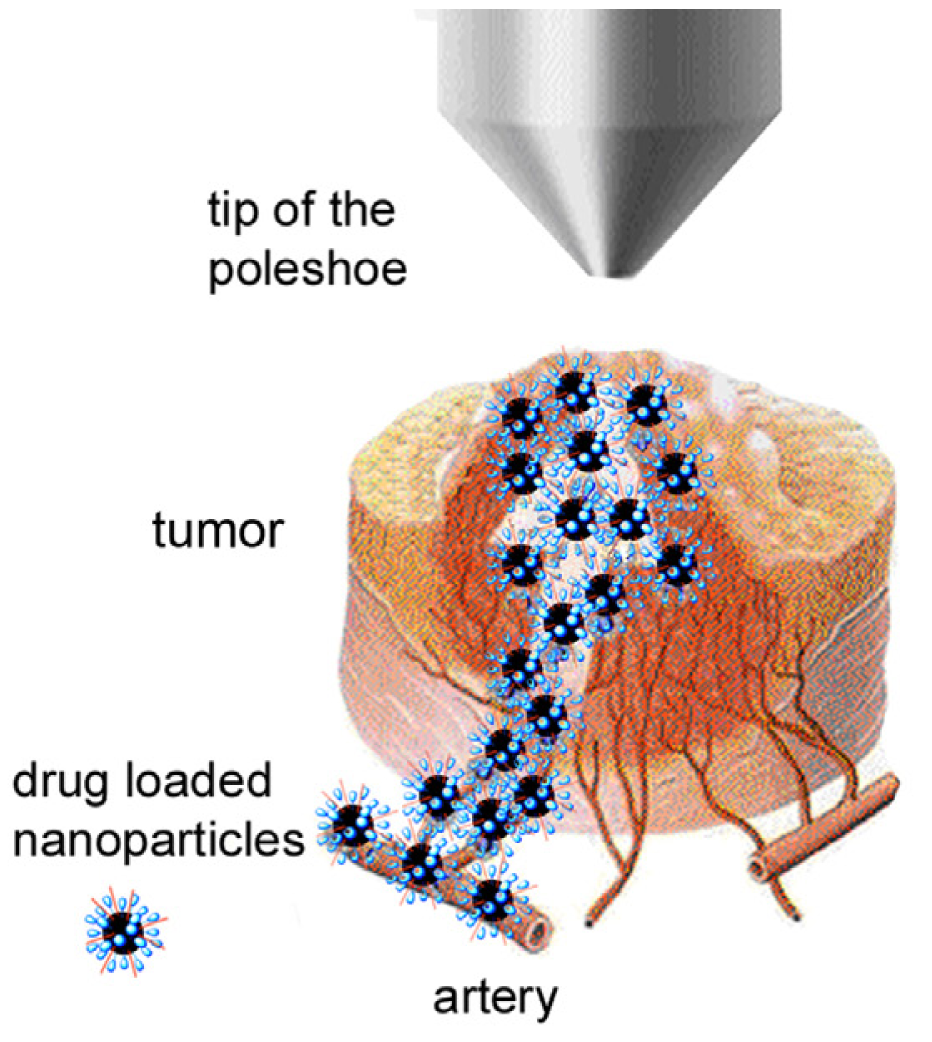
\includegraphics[scale=.7]{DrugTarget.png}
			\end{figure}
		\end{minipage}%
	\end{itemize}
\end{frame}

\section{PDE Model for Two--Phase Ferrofluid Flows}
\begin{frame}{PDE Model for Two--Phase Ferrofluid Flow}
	\begin{itemize}
		\item Dr. Nochetto and collaborators developed a model for two--phase ferrofluid flows and devised an energy stable numerical scheme \cite{DiffuseInterface}.
		\vspace{.1in}
		\item The model was not derived, but instead was assembled.
		\vspace{.1in}
		\item Important results from \cite{DiffuseInterface}:
		\begin{itemize}
			\item Proved an energy law for the PDE model.
			\item Proved the numerical scheme was energy stable and the existence of a local solution.
			\item For an even simpler model, they proved stability, convergence, and the existence of solutions.
		\end{itemize}
	\end{itemize}
\end{frame}

\subsection{Cahn--Hilliard Equation}
\begin{frame}{Modeling a Two--Phase Fluid}
\begin{itemize}
	\item In order to track both fluids, a diffuse interface is used.
	\item The phase variable $\theta$ is introduced, which takes values in $[-1,1]$.
	\item The evolution of $\theta$ is given by a modified Cahn--Hilliard equation:
	\vspace{.1in}\\
	\begin{minipage}{.5\paperwidth}
		$$
		\left\{
		\begin{aligned}
		\theta_t + \diverg(\mathbf{u}\theta) + \gamma \lap \psi &= 0 &\text{in }\Omega \\
		\psi - \eps \lap \theta + \frac{1}{\eps}f(\theta) &= 0 & \text{in }\Omega \\
		\partial_\eta \theta = \partial_\eta\psi &= 0 & \text{on }\Gamma,
		\end{aligned}
		\right.
		$$
		where
		\begin{itemize}
			\item $0 < \eps << 1$ is related to the interface thickness,
			\item $\gamma >0$ is the constant mobility,
			\item $\psi$ is the chemical potential,
			\item $f(\theta)$ is the truncated double well potential.
		\end{itemize}
	\end{minipage}%
	\begin{minipage}{.3\paperwidth}
		\begin{figure}[!b]
			\centering
			
			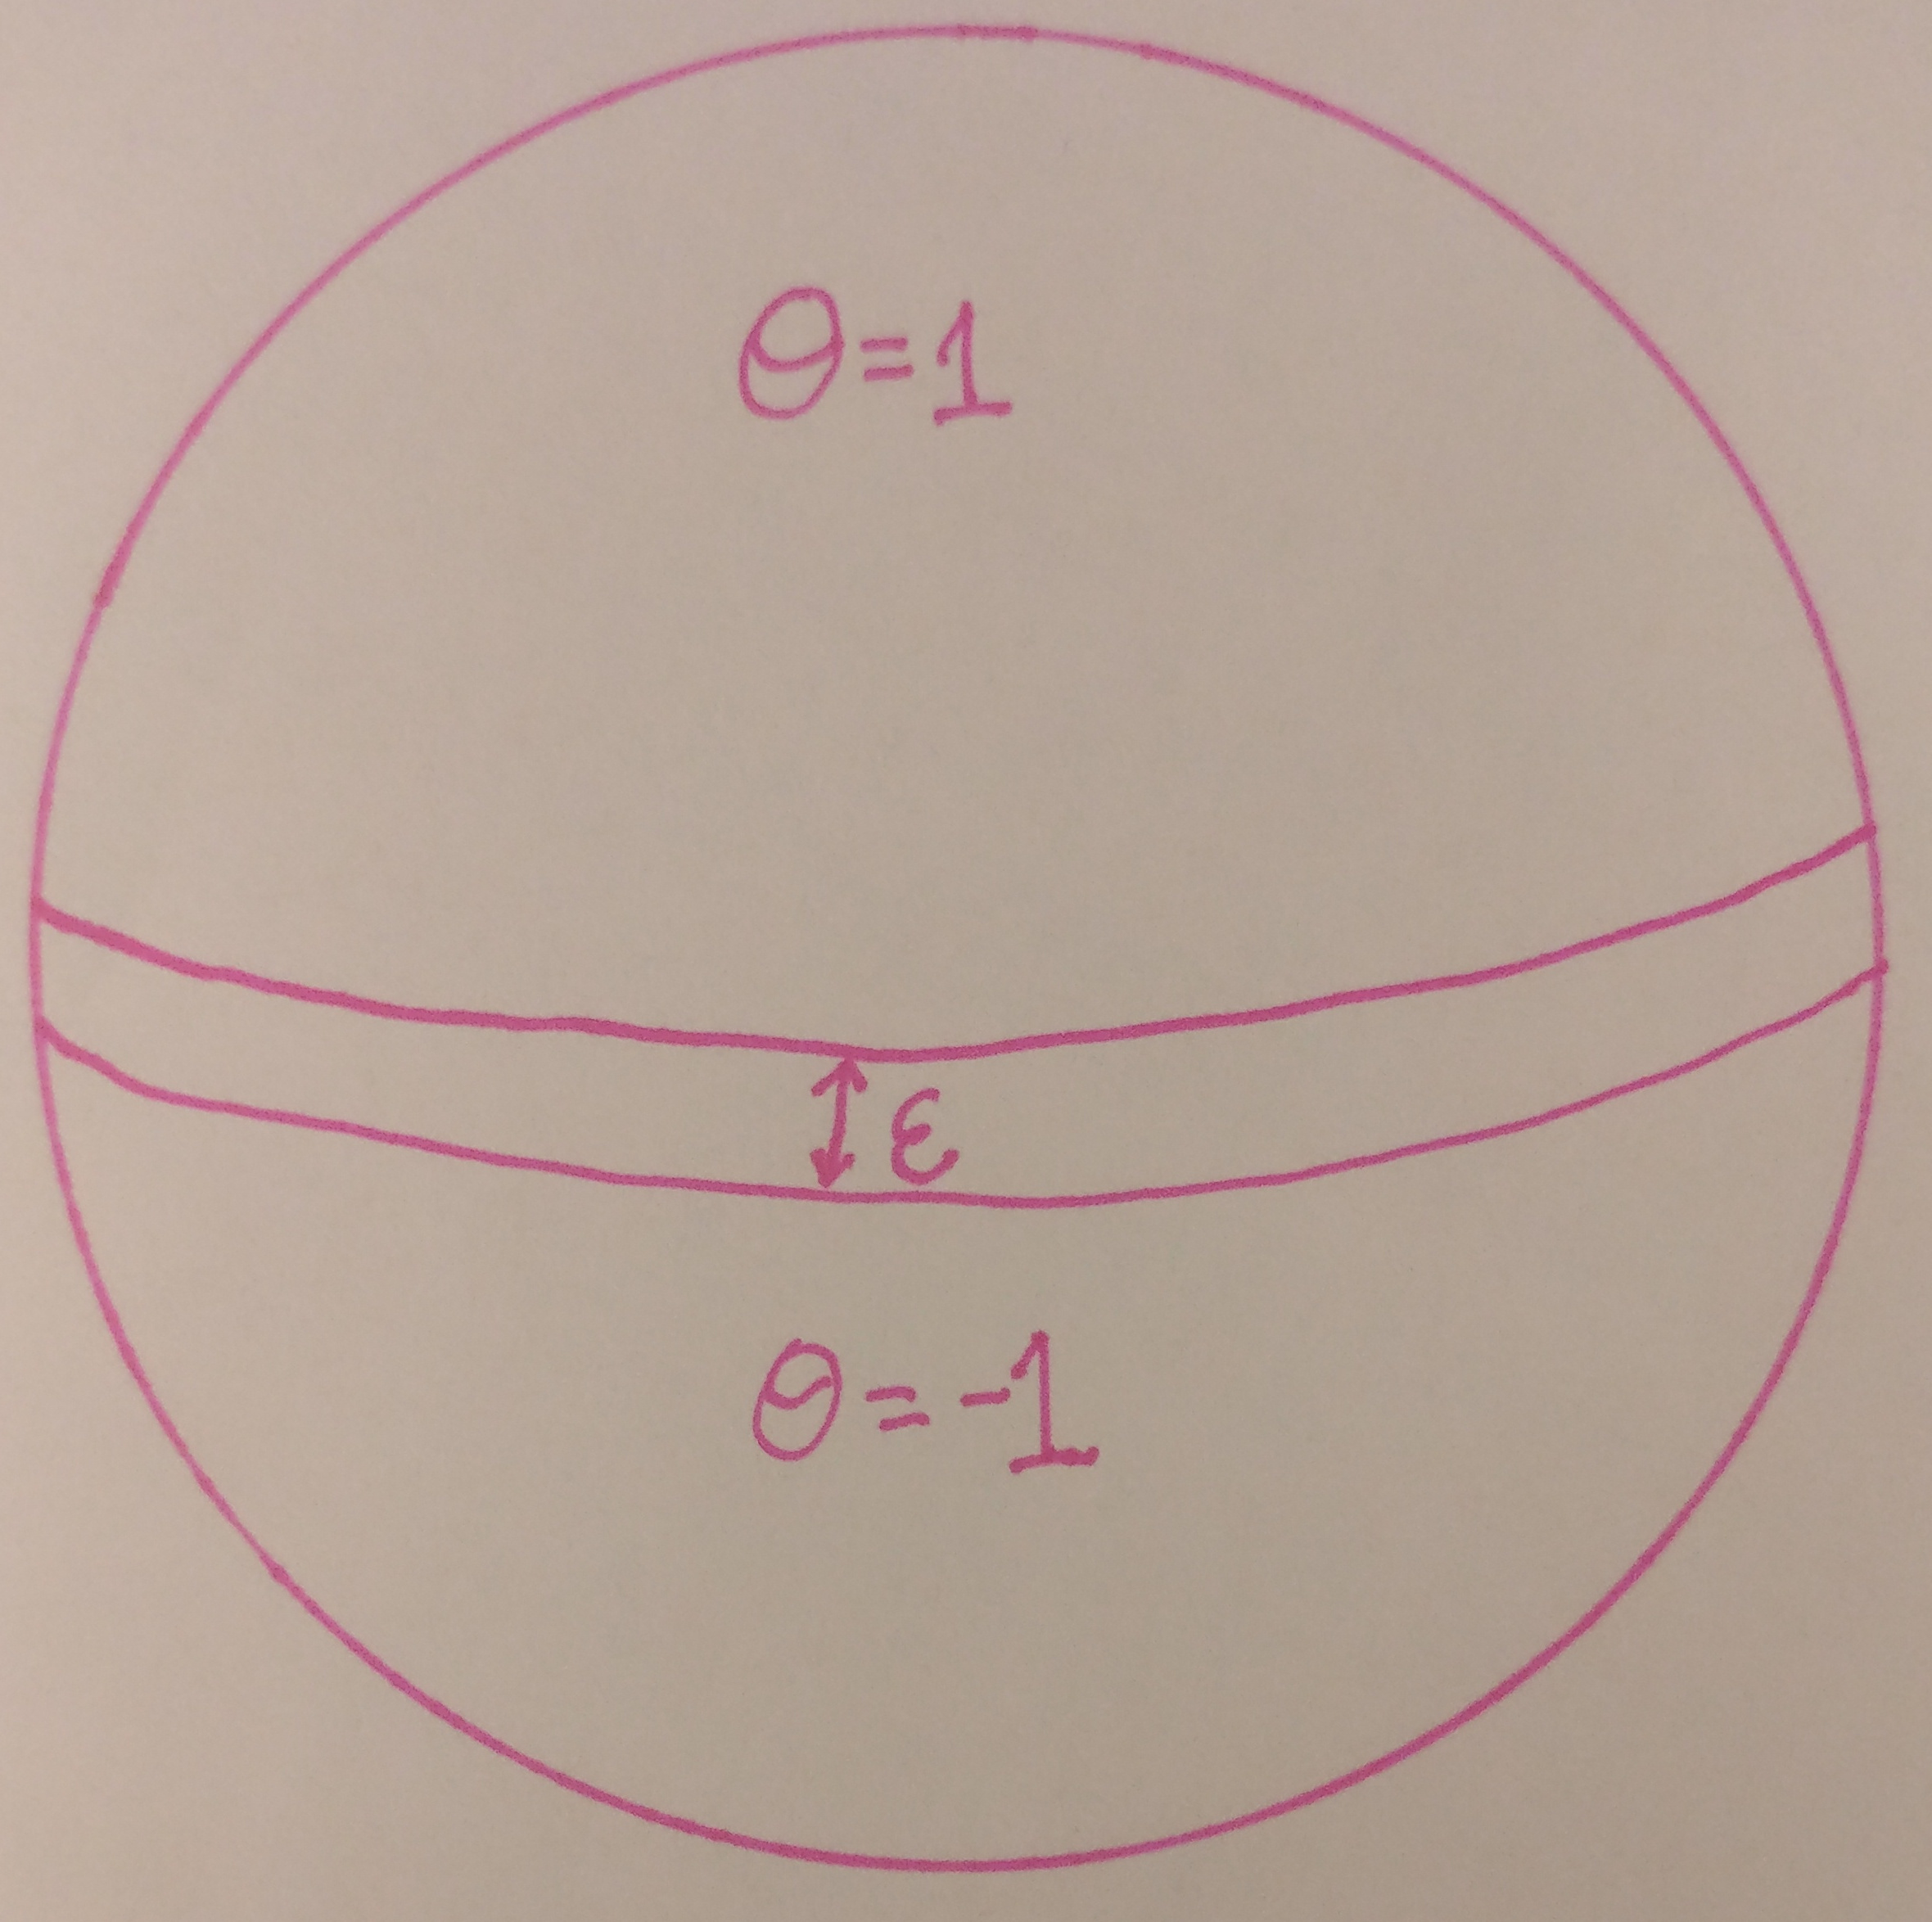
\includegraphics[scale=.05]{CahnHilliard.jpg}
		\end{figure}
	\end{minipage}%
\end{itemize}
\end{frame}

\subsection{Magnetic Field Equations}
\begin{frame}{Modeling of the Magnetic Field}
\begin{itemize}
	\item Instead of using the magnetostatics equations, a simplified approach was used.
	\item Define the magnetic field by 
	$$
		\mathbf{h} := \mathbf{h}_a + \mathbf{h}_d,
	$$
	where 
	\begin{itemize}
		\item $\mathbf{h}_a$ -- smooth harmonic (curl--free and $\diverg$--free) applied magnetizing field,
		\item $\mathbf{h}_d$ -- demagnetizing field.
	\end{itemize}
	\item Then the magnetic field is induced via the scalar potential $\varphi$ by
	$$
		\mathbf{h} = \grad\varphi,
	$$
	along with,
	$$
		-\lap \varphi =\diverg(\mathbf{m}-\mathbf{h}_a) \quad \text{in }\Omega,\quad \quad \partial_\eta\varphi = (\mathbf{h}_a - \mathbf{m})\cdot\eta \quad \text{on }\Gamma.
	$$
\end{itemize}
\end{frame}

\subsection{Ferrohydrodynamics Equations}
\begin{frame}{Modeling of Ferrohydrodynamics}
\begin{itemize}
	\item A simplified version of Shliomis model is used, which couples an advection--reaction equation for the magnetization $\mathbf{m}$:
	$$
		\mathbf{m}_t + (\mathbf{u}\cdot \grad)\mathbf{m}=-\frac{1}{\mathscr{T}}(\mathbf{m} - \varkappa_\theta\mathbf{h}),
	$$
	with the Navier--Stokes equations of incompressible fluids for the velocity--pressure pair $(\mathbf{u},p)$:
	\begin{align*}
		\mathbf{u}_t + (\mathbf{u}\cdot\grad)\mathbf{u} - \diverg (\nu_\theta \mathbf{T(u)}) + \grad p &= \mu_0(\mathbf{m}\cdot \grad)\mathbf{h} + \frac{\lambda}{\eps}\theta\grad \psi,\\
		\diverg \mathbf{u} &= 0,
	\end{align*}
	where
	\begin{itemize}
		\item $\mathscr{T}$ is the relaxation time of the ferrofluid,
		\item $\varkappa_\theta$ is the magnetic susceptibility of the phase variable,
		\item $\nu_\theta$ is the viscosity of the phase variable,
		\item $\mu_0$ is the constitutive parameter related to the Kelvin force,
		\item $\frac{\lambda}{\eps}\theta\grad \psi$ is the capillary force.
	\end{itemize}
	\item This is supplemented with a no--slip condition on the boundary:
	$$
		\mathbf{u} = 0 \quad \text{on }\Gamma. 
	$$
\end{itemize}
\end{frame}

\subsection{Full Model}
\begin{frame}
\begin{itemize}
	\item The model reads: Consider a bounded convex polygon/polyhedron domain $\Omega\subset \Real^d$ ($d=2$ or $3$) with boundary $\Gamma$. The evolution of the system is given by the following set of equations in strong form in $\Omega$
	\begin{subequations}\label{Model}
		\begin{align}
		\label{Cahn-Hilliard:1}\theta_t + \diverg(\mathbf{u}\theta) + \gamma \lap \psi &= 0,\\
		\label{Cahn-Hilliard:2}\psi - \eps \lap \theta + \frac{1}{\eps}f(\theta) &= 0,\\
		\label{Advection-Reaction}\mathbf{m}_t + (\mathbf{u}\cdot \grad)\mathbf{m}&=-\frac{1}{\mathscr{T}}(\mathbf{m} - \varkappa_\theta\mathbf{h}),\\
		\label{MagScalarPot}-\lap \varphi &=\diverg(\mathbf{m}-\mathbf{h}_a),\\
		\label{NavierStokes}\mathbf{u}_t + (\mathbf{u}\cdot\grad)\mathbf{u} - \diverg (\nu_\theta \mathbf{T(u)}) + \grad p &= \mu_0(\mathbf{m}\cdot \grad)\mathbf{h} + \frac{\lambda}{\eps}\theta\grad \psi,\\
		\label{DivFree}\diverg \mathbf{u} &= 0,
		\end{align}
	\end{subequations}
	for every $t\in[0,t_F]$, where $\mathbf{T(u)}=\frac{1}{2}(\grad \mathbf{u} + \grad\mathbf{u}^T)$ denotes the symmetric gradient and $\mathbf{h}=\grad \varphi$. The system (\ref{Model}) is supplemented with the boundary conditions
	\begin{equation}\label{ModelBC}
	\partial_\eta \theta = \partial_\eta\psi = 0,\quad \mathbf{u}=0,\quad\text{and}\quad \partial_\eta\varphi = (\mathbf{h}_a - \mathbf{m})\cdot\eta \quad \text{on }\Gamma.
	\end{equation}
\end{itemize}
\end{frame}

\section{Numerical Method}
\begin{frame}
	Define the backward difference operator $\delta f^k = f^k - f^{k-1}$.\\
	\vspace{.1in}
	For given smooth initial data $\set{\Theta^0, \mathbf{M}^0,\mathbf{U}^0}$ and timestep $\tau$, compute $\set{\Theta^k, \Psi^k, \mathbf{M}^k, \Phi^k, \mathbf{U}^k, {P}^k}\in \mathbb{G}_h\times \mathbb{Y}_h\times \mathbb{M}_h\times\mathbb{X}_h\times\mathbb{U}_h\times\mathbb{P}_h$ for every $k\in\set{1,...,K}$ that solves
	
	\footnotesize\begin{subequations}\label{NumScheme}
		\begin{align}
		\label{NumScheme:1}\bigg(\frac{\delta\Theta^k}{\tau}, \Lambda\bigg) - (\mathbf{U}^k\Theta^{k-1}, \grad\Lambda) - \gamma(\grad \Psi^k, \grad \Lambda)&=0,\\
		\label{NumScheme:2}(\Psi^k, \Upsilon) + \eps(\grad \Theta^k, \grad \Upsilon) + \frac{1}{\eps}(f(\Theta^{k-1}), \Upsilon) + \frac{1}{\eta}(\delta\Theta^k, \Upsilon) &= 0,\\
		\label{NumScheme:3}\bigg(\frac{\delta\mathbf{M}^k}{\tau}, \mathbf{Z}\bigg) - \mathcal{B}_h^m(\mathbf{U}^k, \mathbf{Z}, \mathbf{M}^k) + \frac{1}{\mathscr{T}}(\mathbf{M}^k, \mathbf{Z}) &= \frac{1}{\mathscr{T}}(\varkappa_\theta\mathbf{H}^k, \mathbf{Z}),\\
		\label{NumScheme:4}(\grad\Phi^k, \grad X) &= (\mathbf{h}_a^k - \mathbf{M}^k, \grad X),\\
		\begin{split}
		\label{NumScheme:5}\bigg(\frac{\delta\mathbf{U}^k}{\tau}, \mathbf{V}\bigg) + \mathcal{B}_h(\mathbf{U}^{k-1}, \mathbf{U}^k, \mathbf{V}) + (\nu_\theta\mathbf{T(U}^k), \mathbf{T(V)}) - (P^k, \diverg \mathbf{V}) &= \mu_0\mathcal{B}_h^m(\mathbf{V}, \mathbf{H}^k, \mathbf{M}^k)\\
		&\phantom{{}={}}+\frac{\lambda}{\eps}(\Theta^{k-1}\grad \Psi^k, \mathbf{V}),
		\end{split}\\
		\label{NumScheme:6}(Q, \diverg\mathbf{U}^k) &= 0.
		\end{align}
	\end{subequations}
	\normalsize
\end{frame}

\section{Numerical Implementation}
\begin{frame}{Numerical Implementation Details}

Discretization of the Numerical Scheme:
\begin{itemize}
	\item Time Discretization: Backward Euler is used.
	\item Space Discretization: A mix of Continuous and Discontinuous Galerkin is used, approximating the spaces with polynomials of degree $2$ in each variable (i.e. $\mathcal{Q}_2$ elements).
	\begin{itemize}
		\item Continuous: Cahn--Hilliard, Magnetic potential, and Navier Stokes equations.
		\item Discontinuous: Magnetization equations.
	\end{itemize}
\end{itemize}

Fixed Point Solver:
\begin{itemize}
	\item A Picard--like iteration is used.
	\item Utilizes the "lagging" of the velocity $\mathbf{U}$ to solve each subsystem.
	\item Iterates until a fixed point for $\mathbf{U}^k$ is reached.
	\item Given $\mathbf{U}^{k-1}$ 
	\begin{itemize}
		\item[1)] Compute $\Theta^k$ and $\Psi^k$ substituting $\mathbf{U}^{k-1}$ for $\mathbf{U}^{k}$.
		
		\item[2)] Next compute $\mathbf{M}^k$ and $\Phi^k$ using $(\Theta^k,\Psi^k)$ from the previous iteration and substituting $\mathbf{U}^{k-1}$ for $\mathbf{U}^{k}$.
		
		\item[3)] Finally, compute $\mathbf{U}^k$ and $P^k$ using $(\Theta^k,\Psi^k, \mathbf{M}^k, \Phi^k)$ from the previous two iterations.
		
		\item[4)] Repeat steps 1-3 using $\mathbf{U}^k$ from the previous iteration as input until $\mathbf{U}^k$ does not change between iterations.
	\end{itemize}
\end{itemize}
\end{frame}

\section{Semester Plan}
\begin{frame}{Semester Plan}
	\begin{itemize}
		\item Implement and unit test solvers for each subsystem in "isolation".
		\vspace{.1in}
		\begin{itemize}
			\item Cahn--Hilliard (\ref{NumScheme:1})--(\ref{NumScheme:2})
			\vspace{.1in}
			\item Navier--Stokes (\ref{NumScheme:5})--(\ref{NumScheme:6})
			\vspace{.1in}
			\item Magnetization (\ref{NumScheme:3})--(\ref{NumScheme:4})
		\end{itemize}
		\vspace{.1in}
		\item Combine the solvers using a Picard iteration to implement the full two phase ferrofluid flow.
	\end{itemize}
\end{frame}

\section{Adaptive Refinement}
\begin{frame}{Adaptive Mesh Refinement}
	For adaptive refinement, we used a method of marking cells for refinement known as Dofler marking. Our adaptive refinement procedure is:
	\begin{itemize}
		\item Compute the element indicator $\eta_T$ on each element, where 
		$$
			\eta_T^2 = h_T\int_{\partial T}\abs{\bigg\llbracket\frac{\partial \Theta}{\partial \eta}\bigg\rrbracket}^2dS \quad \forall T\in\mathcal{T}_h,
		$$
		and $\llbracket\cdot\rrbracket$ is the jump across the face.
		\item Order the elements from highest to lowest based on their element indicator value.
		\item Compute the set of elements whose error makes up $55$ percent of the total error for refinement, starting with the higher valued elements.
		\item Compute the set of elements whose error makes up $5$ percent of the total error for coarsening, starting with the lowered valued elements.
		\item Refine/coarsen the mesh and transfer the solution from the old mesh to the new mesh.
	\end{itemize}
	We enforce a limit on the number of times an element can be refined. This procedure is performed every 5 iterations and on the initial condition.
\end{frame}

\section{Solving Cahn--Hilliard}
\begin{frame}{Cahn--Hilliard Matrix Structure}
	\begin{itemize}
		\item Rearranging the system we have that
		\begin{align*}
			\bigg(\Theta^k, \Lambda\bigg) - \tau\gamma(\grad \Psi^k, \grad \Lambda)&=\bigg(\Theta^{k-1}, \Lambda\bigg) + \tau(\mathbf{U}^k\Theta^{k-1}, \grad\Lambda),\\
			(\Psi^k, \Upsilon) + \eps(\grad \Theta^k, \grad \Upsilon) + \frac{1}{\eta}(\Theta^k, \Upsilon) &= \frac{1}{\eta}(\Theta^{k-1}, \Upsilon)-\frac{1}{\eps}(f(\Theta^{k-1}), \Upsilon).\\
		\end{align*}
		
		\item This leads to the following block matrix form
		$$\begin{pmatrix}
			M & -\tau\gamma K \\
			\eps K + \frac{1}{\eta}M & M
		\end{pmatrix}
		\begin{pmatrix}
			\Theta^k\\
			\Psi^k
		\end{pmatrix} = 
		\begin{pmatrix}
			f\\
			g
		\end{pmatrix},
		$$
		where $M$ and $K$ are the usual mass and stiffness matrices and $f$ and $g$ are the respective right hand sides.
	\end{itemize}
\end{frame}

\begin{frame}{Reduced Phase System}
	\begin{itemize}
		\item We eliminate the chemical potential by adding $\tau\gamma KM^{-1}$ the second row to the first. 
		\vspace{.1in}
		\item Doing so yields the following reduced phase system
		$$
			\bigg(M + \tau\eps\gamma KM^{-1}K + \frac{\tau \gamma}{\eta}K\bigg)\Theta^k = f + \tau \gamma KM^{-1}g.
		$$
		\vspace{.1in}
		\item The chemical potential is then found by solving
		$$
			M \Psi^k = g - \bigg(\eps K + \frac{1}{\eta}M\bigg)\Theta^k.
		$$
	\end{itemize}
\end{frame}

\begin{frame}{Solving the Reduced Phase System}
	\begin{itemize}
		\item In order to precondition the reduced phase system, we consider the following preconditioner
		$$
			P = M + \tau\gamma\eps K\text{diag}(M)^{-1}K + \tau\frac{\gamma}{\eta}K.
		$$
		\item When solving with GMRES, we then use an incomplete LU preconditioner of the preconditioner matrix $P$.
		
		\item Note: We never explicitly compute the matrix $M + \tau\eps\gamma KM^{-1}K + \frac{\tau \gamma}{\eta}K$. When solving with GMRES, you only need the action of the matrix. This allows us to not compute the inverse of $M$ as we can compute its action on a vector $x$,
		$$
			y = M^{-1}x,
		$$
		by solving
		$$
			My = x
		$$
		using CG.
		\item Finally, we solve for the chemical potential using CG by using the action of the inverse of $M$.
	\end{itemize}
\end{frame}

\begin{frame}{Cahn--Hilliard Solver Verification}
	We verify the solver using three unit tests.
	\vspace{.1in}
	\begin{itemize}
		\item[1)] A flat initial profile with no forcing and adaptive refinement.
			\vspace{.1in}
		\item[2)] A circular profile with no forcing and adaptive refinement.
			\vspace{.1in}
		\item[3)] A forced solution on a series of globally refined grids. This is done to compute the convergence rate.
	\end{itemize}
\end{frame}

\begin{frame}
	The initial condition for the flat profile was
	$$
		f(x, y) = \begin{cases}
			-1 & y > .06\\
			1 & \text{otherwise}
		\end{cases}.
	$$
	The maximum level of refinement was 5 and the initial data was refined 20 times. Model parameters were chosen as $\eps = .001$, $\gamma = .2$, $\eta = .000001$. The error of the solution stayed approximately constant over 1000 time steps.
	\begin{minipage}{.4\paperwidth}
		\begin{figure}[!b]
			\centering
			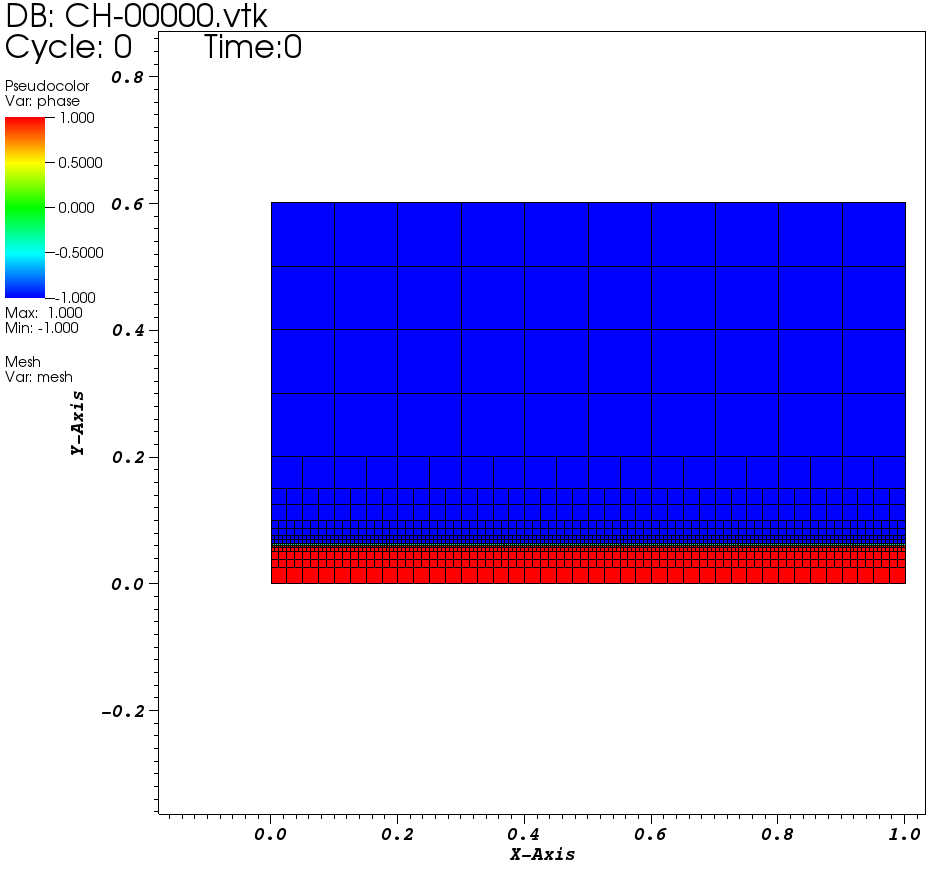
\includegraphics[scale=.6]{CHFlat1.png}
			\caption*{Time step 0}
		\end{figure}
	\end{minipage}%
	\begin{minipage}{.4\paperwidth}
		\begin{figure}[!b]
			\centering
			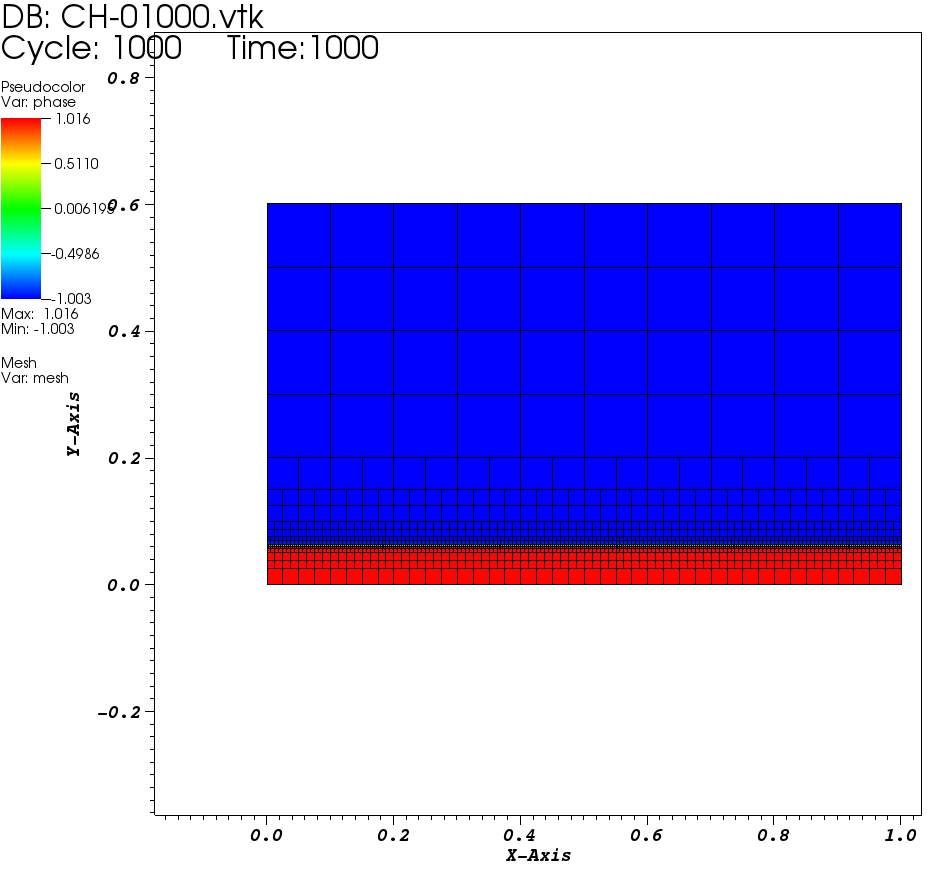
\includegraphics[scale=.6]{CHFlat2.png}
			\caption*{Time step 1000}
		\end{figure}
	\end{minipage}
\end{frame}

\begin{frame}
The initial condition for the circular profile was
$$
f(x, y) = \begin{cases}
-1 & (x,y)\in B((.5, .3), .2)\\
1 & \text{otherwise}
\end{cases}.
$$
The maximum level of refinement was 5 and the initial data was refined 20 times. Model parameters were chosen as $\eps = .001$, $\gamma = .2$, $\eta = .000001$. The error of the solution stayed approximately constant over 1000 time steps.
\begin{minipage}{.4\paperwidth}
	\begin{figure}[!b]
		\centering
		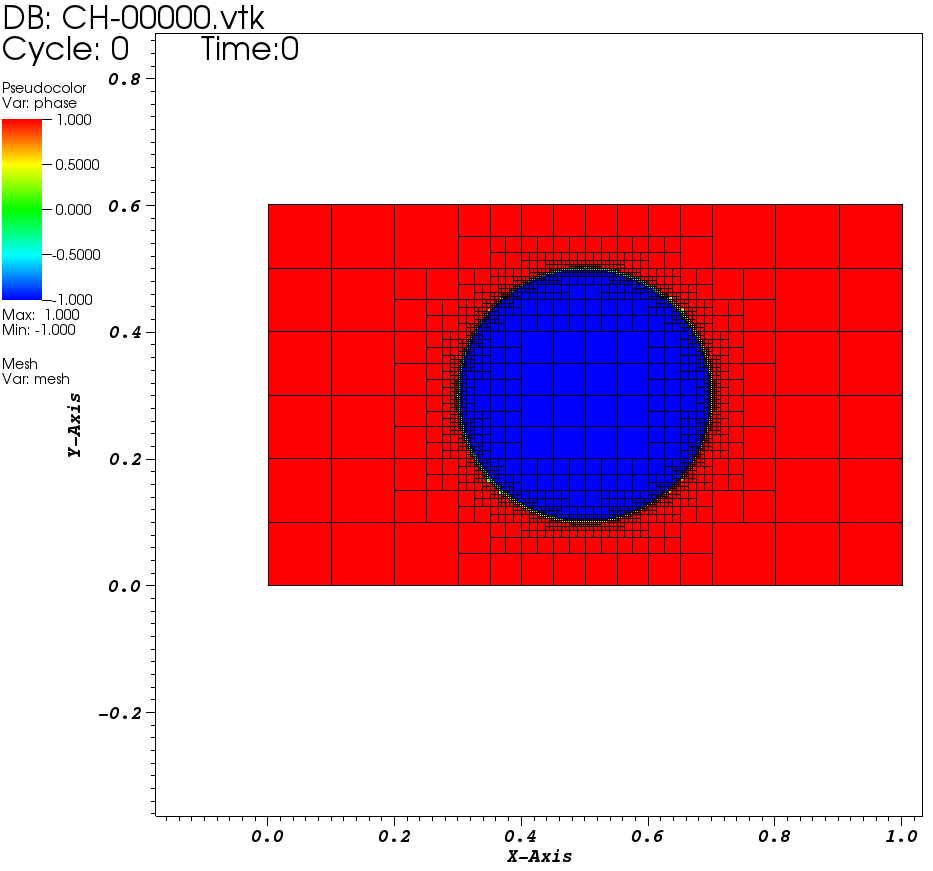
\includegraphics[scale=.6]{CHBall1.png}
		\caption*{Time step 0}
	\end{figure}
\end{minipage}%
\begin{minipage}{.4\paperwidth}
	\begin{figure}[!b]
		\centering
		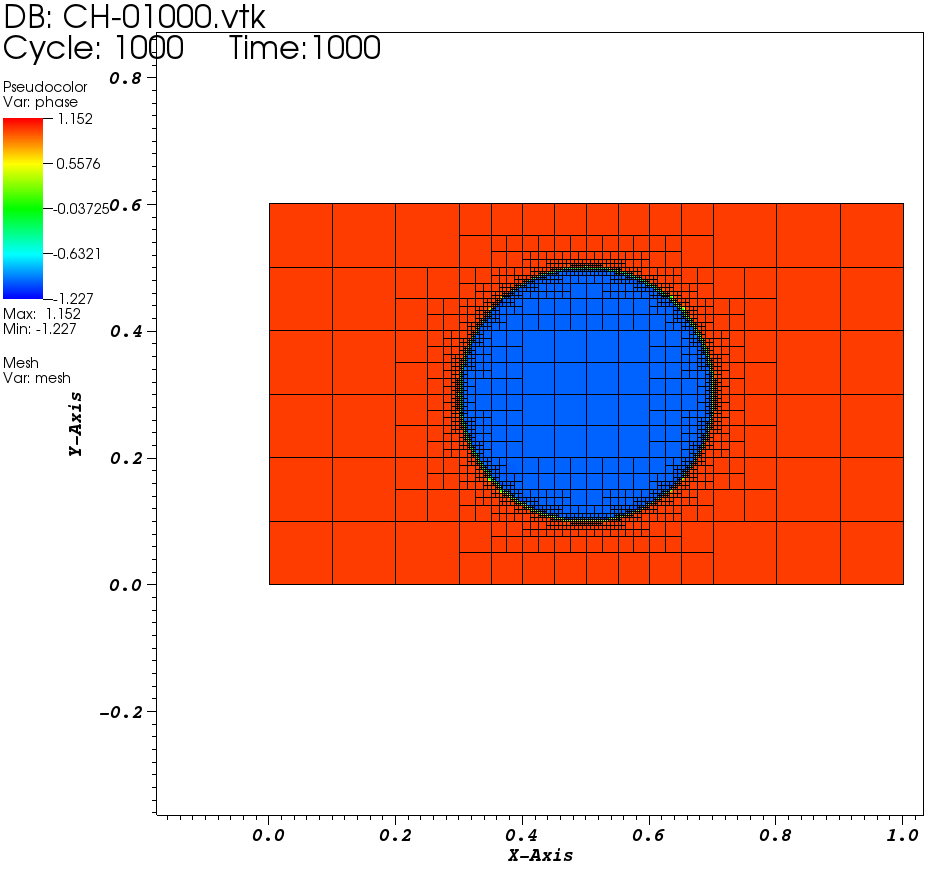
\includegraphics[scale=.6]{CHBall2.png}
		\caption*{Time step 1000}
	\end{figure}
\end{minipage}
\end{frame}

\begin{frame}
	The forcing function chosen was $f(x,y) = \cos(2\pi x)cos(2\pi y)$ and $\Omega = [-1, 1]^2$. Model parameters were chosen as $\eps = .2$, $\gamma = .2$, $\eta = .000001$. The error was computed after 1000 iterations.
	
	\begin{table}[H]
		\begin{center}
			\begin{tabular}{|c|r|c|c|c|c|c|c|} \hline
				
				\multicolumn{2}{|c|}{n cells} & 
				\multicolumn{3}{|c|}{$H^1$-error} & 
				\multicolumn{3}{|c|}{$L^2$-error}\\ \hline
				2 & 16 & 4.264e+00 & - & - & 3.109e-01 & - & -\\ \hline
				3 & 64 & 8.079e-01 & 5.28 & 2.40 & 2.658e-02 & 11.70 & 3.55\\ \hline
				4 & 256 & 2.038e-01 & 3.96 & 1.99 & 3.310e-03 & 8.03 & 3.01\\ \hline
				5 & 1024 & 5.104e-02 & 3.99 & 2.00 & 4.125e-04 & 8.02 & 3.00\\ \hline
				6 & 4096 & 1.277e-02 & 4.00 & 2.00 & 5.152e-05 & 8.01 & 3.00\\ \hline
			\end{tabular}
		\end{center}
	\end{table}

	This is the convergence rate that we expect for both the $H^1$ and $L^2$ error for $Q_2$ elements.
\end{frame}

\section{Solving Navier--Stokes}
\begin{frame}{Navier--Stokes Block Matrix Structure}
	The system has following block matrix form
	$$\begin{pmatrix}
	F & B^T \\
	B & 0
	\end{pmatrix}
	\begin{pmatrix}
	\mathbf{U}^k\\
	P^k
	\end{pmatrix} = 
	\begin{pmatrix}
	f\\
	0
	\end{pmatrix},
	$$
	where 
	$$
		F = \big(\mathbf{U}^k, \mathbf{V}\big) + \tau\mathcal{B}_h(\mathbf{U}^{k-1}, \mathbf{U}^k, \mathbf{V}) + \tau(\nu_\theta\mathbf{T(U}^k), \mathbf{T(V)}),
	$$
	$$
		B = (Q, \diverg\mathbf{U}^k),
	$$
	and 
	$$
		f = \big(\mathbf{U}^{k-1}, \mathbf{V}\big) + \tau\mu_0\mathcal{B}_h^m(\mathbf{V}, \mathbf{H}^k, \mathbf{M}^k) + \tau\frac{\lambda}{\eps}(\Theta^{k-1}\grad \Psi^k, \mathbf{V}).
	$$
\end{frame}

\begin{frame}
	We would like to use the block preconditioner
	$$
		P = \begin{pmatrix}
		F & 0\\
		B & -S
		\end{pmatrix}
	$$
	where $S$ is the the Schur Complement $S = B^TF^{-1}B$. This preconditioner is desirable as it has the property that
	$$
		P^{-1}\begin{pmatrix}
		F & B^T \\
		B & 0
		\end{pmatrix} = \begin{pmatrix}
		I & F^{-1}B^T \\
		0 & I
		\end{pmatrix}.
	$$
	Since we don't want to compute inverse matrices, we instead consider the following approximation for $P^{-1}$
	$$
		P^{-1} \approx \begin{pmatrix}
		\overset{\sim}{F}^{-1} & 0\\
		\overset{\sim}{S}^{-1}B\overset{\sim}{F}^{-1} & -\overset{\sim}{S}^{-1}
		\end{pmatrix}
	$$
	where $\overset{\sim}{F}^{-1}$ is computed as an inverse action and $\overset{\sim}{S}^{-1}$ is the Least Squares Commutator \cite{Precond} defined as
	$$
	\overset{\sim}{S}^{-1} = \big(B\text{diag}(M)^{-1}B^T\big)^{-1}\big(B\text{diag}(M)^{-1}F\text{diag}(M)^{-1}B^T\big)\big(B\text{diag}(M)^{-1}B^T\big)^{-1},
	$$
	and $M$ is the mass matrix for the velocity.
\end{frame}

\begin{frame}
	The preconditioner was implemented to compute $Y = P^{-1}X$, where $X,Y$ are block vectors. It does so in three steps.
	\begin{itemize}
		\item Compute
		$$
			Y_0 = \overset{\sim}{F}^{-1}X_0.
		$$
		\item Then compute in a temporary vector $N$
		$$
			N = X_1 - BX_0 = X_1 - B\overset{\sim}{F}^{-1}X_0.
		$$
		\item Finally compute
		$$
			Y_1 = S^{-1}N = S^{-1}\big(X_1 - B\overset{\sim}{F}^{-1}X_0\big).
		$$
	\end{itemize}

	Using this preconditioner the system is solved using GMRES.
\end{frame}

\begin{frame}{Navier--Stokes Solver Verification}
	We verify the solver using the following forced solution
	$$
		\mathbf{u}(x,y,t) = \begin{pmatrix}
		t\sin(\pi x)\sin(\pi(y + .5))\\
		t\cos(\pi x)\cos(\pi(y + .5))
		\end{pmatrix}, \quad p(x,y,t) = \sin(2\pi(x - y) + t),
	$$
	on $\Omega = [0,1]^2$.
	The model parameters are $\mu = 1$, $\lambda = .05$, $\eps = .2$. The system was solved until $t=2$ with 1000 time steps. The system was solved on a uniformly refined grid with levels $3, 4, 5$. 
	
	\begin{table}[H]
		\begin{center}
			\begin{tabular}{|c|r|c|} \hline
				
				\multicolumn{2}{|c|}{n cells} &  
				\multicolumn{1}{|c|}{$L^2$-error}\\ \hline
				3 & 64 & 0.642479 \\ \hline
				4 & 256 & 0.642518\\ \hline
				5 & 1024 &  0.64252\\ \hline
			\end{tabular}
		\end{center}
	\end{table}
\end{frame}

\begin{frame}{Deliverables}
	\begin{itemize}
		\item Cahn--Hilliard solver and unit tests
		\item Navier--Stokes solver and unit test
		\item Summary of the capabilities of the code will be published on the github repo
		\item List of software requirements
		\item Instructions on how to run each of the codes and how to alter initial conditions and forcing functions
	\end{itemize}
\end{frame}


\section{References}
\begin{frame}{Figure References}
\begin{itemize}
	\item Slide 1: \url{https://youtu.be/wHZDgSFzQ_s?t=12}
	\item Slide 2:
	\begin{itemize}
		\item \url{https://www.researchgate.net/profile/Vikram\_Raghavan2/post/What\_is\_the\_effect\_of\_magnetic\_field\_on\_alignment\_of\_ferro\_fluid\_droplet/attachment/59d622166cda7b8083a1b9a2/AS\%3A273810673078272\%401442292959057/download/Effect+of+Magnetic+field.jpg}
		\item \url{https://ksr-ugc.imgix.net/assets/003/310/641/f0ef73d1fd99f6aa5d96872168478df4\_original.png?v=1424378871\&w=680\&fit=max\&auto=format\&lossless=true\&s=c183d857603c12de82a71f3139283d9e}
		\item \url{https://opentextbc.ca/chemistry/wp-content/uploads/sites/150/2016/05/CNX\_Che\_11\_05\_Colloid.jpg}
	\end{itemize}
	\item Slide 3: \cite{DrugTarget}
	\item Slide 12: \cite{DiffuseInterface}
	\item Slide 13: \cite{DiffuseInterface}
	\item Slide 18: \cite{DiffuseInterface}
\end{itemize}
\end{frame}

\tiny

\begin{frame}[allowframebreaks]{References}
	\bibliographystyle{siam}
	\bibliography{FinalPresentation}
\end{frame}

\end{document}
